\documentclass[12pt]{article}
\usepackage{sbc-template}
\usepackage{graphicx,url}
\usepackage[brazil]{babel}   
%\usepackage[latin1]{inputenc}  
% Please add the following required packages to your document preamble:
% \usepackage{graphicx}
% Please add the following required packages to your document preamble:
% \usepackage{graphicx}
\sloppy

\title{\textbf{Relatório}: Clusters}

\author{
    Romário Da S. Ferreira\inst{1},
    Luiz David Santin\inst{2},
    Lucas Nakamura\inst{3},
    Rafael Vellozo \inst{4}
}



\address{ Departamento Computação \\
        Universidade Tecnologica Federal do Paraná (UTFPR) 
        -- Medianeira, PR -- Brazil
        \email{{romario,lucasnakamura.1996}@alunos.utfpr.edu.br},
        \email{{luiz-santin@hotmail.com}},
        \email{rafaelldassilveira@gmail.com}
}

\begin{document} 

\maketitle

\section{Indrodução}
\subsection{Objetivos}

Criar e configurar um cluster para realização de trabalho de alto custo computacional para computadores convencionais, realizar testes de ordenação em arquivos de diversas tamanhos, fazendo assim observações sobre os resultados obtidos, onde tem-se como intenção ordenar arquivos com tamanho de linha diversos usando um algoritmo Bubble Sort paralelizado no qual foi disponibilizado na universidade de \textit{Heriot-Watt University} na Scotland, os arquivos contendo os valores a serem ordenados foram gerado por um script na linguagem c, no qual foi possível escolher o tamanho em linha do arquivo, possuindo como saída três arquivos, sendo eles randômico, ordenado e invertido.

\section{Materiais} \label{sec:firstpage}
\subsection{Materiais}

Foram utilizado neste experimento 3 computadores pertencentes a Universidade Tecnológica Federal do Paraná, onde os mesmos
possuem a mesma característica de hardware como descrito na Tabela \ref{tab:computersLabor}, usamos também um switch e três pendrives, bem como o sistema operativo Pelican HPC GNU Linux para criação do cluster.

\begin{table}[]
\centering
\caption{Configuração das máquinas utilizadas no cluster}
\label{tab:computersLabor}
\resizebox{\textwidth}{!}{%
\begin{tabular}{l|llll}
Máquina & Processador & Versão do BIOS & Memória física total: & Placa de Rede \\ \hline
Computador 1 & Intel64 Family 6 Model 42 Stepping 7 GenuineIntel $\sim$3100 Mhz & Dell Inc. A07, 10/09/2011 & 8.073 MB & \begin{tabular}[c]{@{}l@{}}2 NIC(s) instalado(s). \\ {[}01{]}: Intel(R) 82579LM Gigabit Network Connection \\ {[}02{]}: Realtek PCI GBE Family Controller\end{tabular} \\
Computador 2 & Intel64 Family 6 Model 42 Stepping 7 GenuineIntel $\sim$3100 Mhz & Dell Inc. A07, 10/09/2011 & 8.073 MB & \begin{tabular}[c]{@{}l@{}}3 NIC(s) instalado(s). \\ {[}01{]}: Intel(R) 82579LM Gigabit Network Connection \\ {[}02{]}: Realtek PCI GBE Family Controller\end{tabular} \\
Computador 3 & Intel64 Family 6 Model 42 Stepping 7 GenuineIntel $\sim$3100 Mhz & Dell Inc. A07, 10/09/2011 & 8.073 MB & \begin{tabular}[c]{@{}l@{}}2 NIC(s) instalado(s). \\ {[}01{]}: Intel(R) 82579LM Gigabit Network Connection \\ {[}02{]}: Realtek PCI GBE Family Controller\end{tabular}
\end{tabular}%
}
\end{table}


\subsection{Metódos}
    Para realização do cluster foi utilizado um sistema operacional próprio para tal tarefa, 
    assim sendo usamos os sistema operacional Pelican HPC GNU Linux, onde realizamos a instalação
    em um pendrive e o tornamos bootavél, partimos do principio da necessidade de existir um computador
    mestre e outros escravos, então assim o fizemos, iniciamos o computador mestre e o configuramos para que
    permitisse que os computadores escravos conectassem ao mestre, no início possuímos problemas com a conexão dos 
    nós escravos com o mestre, mas este problema foi corrigido realizando a configuração correta, então foi necessário 
    que realizássemos a configuração na BIOS de cadas computador escravo para que realizasse o boot via rede, está etapa fez com que 
    os problemas ocorridos com criptografia e permissões fossem evitados. Utilizamos o switch pois ele não é um servidor DHCP, caso
    fosse um servidor DHCP poderia ocasionar problemas no cluster, visto que o nó master é responsável por realizar a distribuição e gerenciamento dos ips.
   
    Foi configurada a inicialização dos três computadores utilizados neste experimento, onde o dois computadores
    escravos foram configurados para inicializar pela placa de rede NIC, enquanto o computador mestre foi configurado
    para inicializar pelo pendrive. Desta forma, quando o computador mestre inicializou pelo pendrive e carregou o sistema
    operacional, foi necessário realizar uma pequena configuração indicando em qual rede o cluster seria montado, permitindo
    que os computadores escravos carregassem o sistema operacional pela rede e evitando a necessidade de criar novos pendrives
    bootavéis para carregar o sistema.

    Necessitou-se realizar a compilação do algoritmo de ordenação e algoritmo de geração de arquivos a serem ordenados. Para isso, utilizou-se o compilador mpicc, o qual é especifico para compilar códigos paralelizados desenvolvidos em c. Também foi necessário fornecer parâmetros de entrada para que a compilação obtivesse sucesso, utilizar o compilador padrão gcc para realizar a compilação do programa que gera arquivos. Como exemplo, temos o comando \textbf{gcc program.c -o programResult}.

    Após realizado todo esse processo, realizou-se a execução de ambos programas. Primeiro gerou-se os arquivos necessários com tamanhos de 500000 e 100000 de linhas, depois foi executado o comando \textbf{mpirun -np num-processos program file-in file-out}, onde váriamos o número de processo de 16 até 256, após a variação de processos realizamos o desligamento 1 máquinas assim ficando com 2 máquinas ligadas e realizamos novamente o teste nos arquivos com 500000 linhas, após a conclusão da tarefa desligamos outra máquina assim ficando com somente uma ativa no cluster e voltamos a realizar o teste.
    
    
    \begin{figure}[!htb]
         \centering
         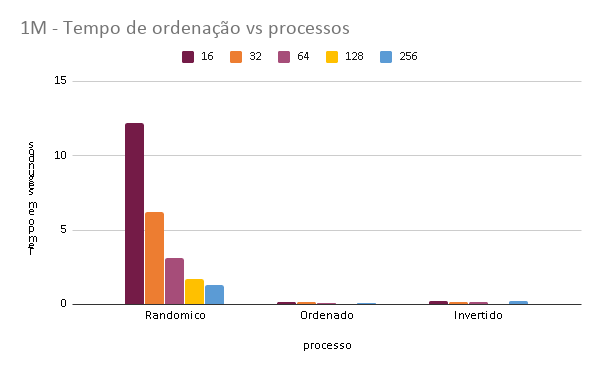
\includegraphics[scale=.5]{chart/chart1.png}
         \caption{Apresenta os tipos de arquivos ordenados de acordo com cada processo vs o tempo consumido para realizar a tarefa, onde os arquivos possuem o tamanho de 1 Milhão de linhas.}
         \label{img:chart1}
    \end{figure}
   
    \begin{figure}[!htb]
         \centering
         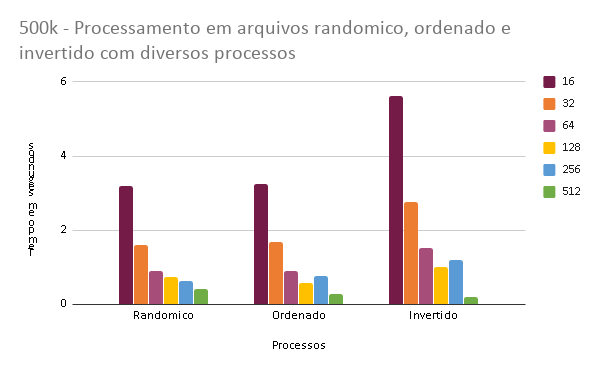
\includegraphics[scale=.5]{chart/chart2.png}
         \caption{Apresenta os tipos de arquivos ordenados de acordo com cada processo vs o tempo consumido para realizar a tarefa, onde os arquivos possuem 500 mil linhas.}
         \label{img:chart2}
    \end{figure}
   
    \begin{figure}[!htb]
         \centering
         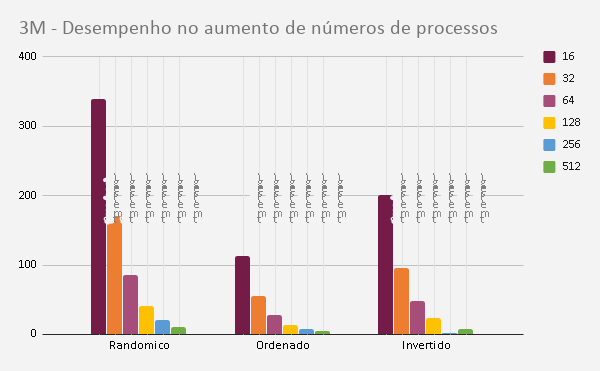
\includegraphics[scale=0.5]{chart/chart3.png}
         \caption{Apresenta os tipos de arquivos ordenados de acordo com cada processo vs o tempo consumido para realizar a tarefa, onde os arquivos possuem 3 Milhões linhas.}
         \label{img:chart3}
    \end{figure}
   
    \begin{figure}[!htb]
         \centering
         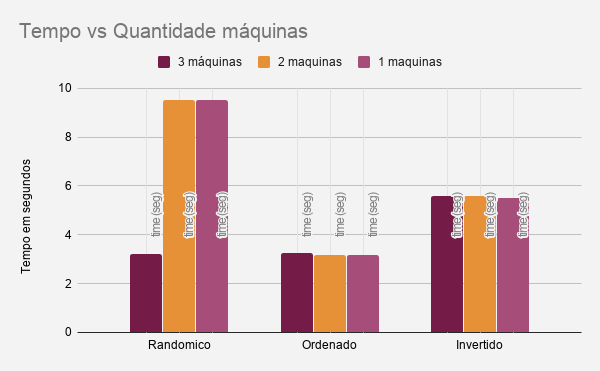
\includegraphics[scale=0.5]{chart/chart4.png}
         \caption{Apresenta os tipos de arquivos ordenados de acordo com um número limitado a 16 processos
         vs o tempo consumido para realizar a tarefa, onde os arquivos possuem 500 mil linhas, neste caso os nós escravos foram desligados no decorrer do teste.}
         \label{img:chart4}
    \end{figure}
   
    
    


\section{Resultados e discussões}

Quando foram utilizadas três máquinas para a ordenar os valores, o arquivo aleatório foi o que mais se destacou pelo fato de que, quando o número de processos era menor, mais rápido foi ordenado, mas quando atingia o número de 512 processos, o desempenho diminuiu. Contudo, utilizando duas máquinas escravas e uma máquina mestra, no total de 16 processos, os valores ficaram maiores apesar de que utilizando apenar uma maquina o desempenho ficou melhor que utilizar duas máquinas, exceto quando tentou ordenar o arquivo randômico, obtendo uma grande redução de desempenho, por requisitar mais do processador. Ao utilizar um algoritmo não paralelizável, o master fazia a utilização de 1 núcleo por vez e assim consumindo muito tempo entre as operações requisitadas.

\begin{table}[]
\begin{tabular}{l|llllll}
           &                 &                     & Tipo de Arquivos  &            &            \\  \hline
           &                 &                     & Tempo em segundos &            &            \\ \hline
        & Linhas     & N. Processos      & Randômico         & Ordenado   & Invertido  \\ \hline
3 maquinas & 3000000    & 16              & 339,132014          & 113,058303        & 200,285386 \\
3 maquinas & 3000000    & 32              & 170,791132          & 55,598693         & 95,987929  &            \\
3 maquinas & 3000000    & 64              & 85,345131           & 27,42872          & 47,990014  &            \\
3 maquinas & 3000000    & 128             & 40,430747           & 13,701426         & 24,039388  &            \\
3 maquinas & 3000000    & 256             & 20,167077           & 7,328713          & 2,608632   &            \\
3 maquinas & 3000000    & 512             & 11,055823           & 5,206665          & 7,890164   &            \\
3 maquinas & 1000000    & 16              & 12,185057           & 0,154966          & 0,254218   &            \\
3 maquinas & 1000000    & 32              & 6,213659            & 0,138077          & 0,162084   &            \\
3 maquinas & 1000000    & 64              & 3,139923            & 0,080498          & 0,154480   &            \\
3 maquinas & 1000000    & 128             & 1,738475            & 0,028435          & 0,037343   &            \\
3 maquinas & 1000000    & 256             & 1,338091            & 0,078705          & 0,208795   &            \\
3 maquinas & 1000000    & 512             & 1,816653            & Erro              & Erro       &            \\
3 maquinas & 500000     & 16              & 3,197146            & 3,240204          & 5,608355   &            \\
3 maquinas & 500000     & 32              & 1,609271            & 1,672758          & 2,753006   &            \\
3 maquinas & 500000     & 64              & 0,892058            & 0,898319          & 1,516231   &            \\
3 maquinas & 500000     & 128             & 0,731357            & 0,566566          & 1,021335   &            \\
3 maquinas & 500000     & 256             & 0,639991            & 0,771383          & 1,204545   &            \\
3 maquinas & 500000     & 512             & 0,408242            & 0,277766          & 0,213484   &            \\
2 maquinas & 500000          & 16                  & 9,499939          & 3,158108   & 5,570042   \\
1 maquinas & 500000          & 16                  & 9,531287          & 3,157503   & 5,493562  
\end{tabular}
\caption{Tabela dos resultados obtidos ao processar os arquivos no cluster}
\label{tab:table-result-cluster}
\end{table}
\section{Conclusões}
Concluiu-se que a utilização do cluster é viável para grandes volumes de dados 
podendo assim substituir um super computador e sendo mais eficiente em alguns casos. 

\bibliographystyle{sbc}

\bibliography{sbc-template}

Pelican HPC Disponivel em: https://www.pelicanhpc.org/download.html 
Acesso: Novembro de 2019

Tutorial Cluster em Pelican Disponivel em: https://www.pelicanhpc.org/tutorial/pelicantutorial.html 
Acesso: Novembro de 2019

Cluster Pelican Disponivel em: http://www.linuxnewmedia.com.br/images/uploads/pdf_aberto/LM_57_48_53_06_tut_pelican.pdf 
Acesso: Novembro de 2019

\end{document}
